% =============================================================================
% Lecture 13: Synthesis — What Twelve Weeks of Forecasting Taught Us
% ECON 8310: Business Forecasting
% University of Nebraska at Omaha
% =============================================================================

\documentclass[aspectratio=169, 11pt]{beamer}

\input{header}

\title[Synthesis]{Synthesis: What the Results Taught Us}
\subtitle{ECON 8310: Business Forecasting --- Lecture 13}
\author{Department of Economics}
\institute{University of Nebraska at Omaha}

% =============================================================================
\begin{document}
% =============================================================================

\begin{frame}
  \titlepage
\end{frame}

\begin{frame}{Lecture Outline}
  \tableofcontents
\end{frame}

% =============================================================================
\section{What We Built}
% =============================================================================

\sectionslide{What We Built}{%
  Twelve weeks, four families of method, and one dataset
  carried through all of them.}

% --- Slide: the arc -----------------------------------------------------------
\begin{frame}{The Arc of the Course}
  \begin{center}
    {\small
    \begin{tabular}{p{2.3cm}p{3.0cm}p{7.0cm}}
      \toprule
      \textbf{Part} & \textbf{Lectures} & \textbf{The central idea} \\
      \midrule
      Time series & 1--3 & Specify a structure --- level, trend, season --- and estimate it. \\[3pt]
      Trees & 4--6 & Stop specifying. Hand an algorithm features and let it find the structure. \\[3pt]
      Deep learning & 7--9 & Let the \emph{architecture} encode what kind of structure to expect. \\[3pt]
      Bayesian & 10--12 & Change the deliverable: return a distribution, not a number. \\
      \bottomrule
    \end{tabular}
    }
  \end{center}

  \vspace{0.1cm}
  Read down that last column and the course is not really four toolkits. It is four answers to a
  single question: \textbf{where does the knowledge in a forecast come from?}

  \vspace{0.1cm}
  From you, in the model structure. From the data, via a search procedure. From the
  architecture's assumptions. Or from a prior, stated openly and updated. \textbf{That framing is
  what survives when the libraries change.}
\end{frame}

% --- Slide: the scoreboard ------------------------------------------------------
% Figure: scripts/figures/lecture13_figures.py (scoreboard). Every number is recomputed there.
% The table stays: scripts/check-book-claims.py reads the book preface's ranking claims from it.
\begin{frame}{The Scoreboard}
  Every model in this course, on the M5 weekly panel --- same 30 series, same held-out block.

  \vspace{0.1cm}
  \begin{columns}[c,onlytextwidth]
    \begin{column}{0.60\textwidth}
      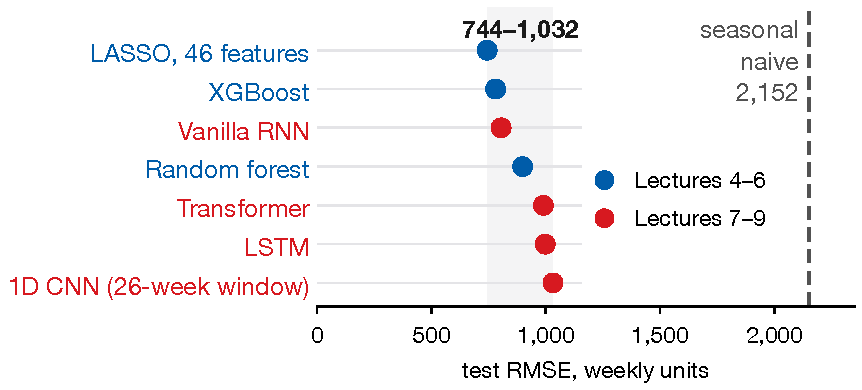
\includegraphics[width=\linewidth]{../Figures/Lecture13_Synthesis/scoreboard.pdf}
    \end{column}
    \begin{column}{0.38\textwidth}
      {\footnotesize
      \setlength{\tabcolsep}{3pt}
      \begin{tabular}{@{}lrl@{}}
        \toprule
        \textbf{Model} & \textbf{RMSE} & \textbf{Where} \\
        \midrule
        LASSO, 46 features & \textbf{744} & HW 4 \\
        XGBoost & 781 & HW 4 \\
        Vanilla RNN & 805 & L9 Part 1 \\
        Random forest & 899 & HW 3 \\
        Transformer & 990 & L9 Part 2 \\
        LSTM & 998 & L9 Part 1 \\
        1D CNN (26-wk) & 1{,}032 & L8 \\
        \midrule
        Seasonal naive & 2{,}152 & benchmark \\
        \bottomrule
      \end{tabular}
      }
    \end{column}
  \end{columns}

  \vspace{0.15cm}
  \textbf{Not the ordering anyone predicts in Week 1.} A 46-coefficient linear model is on top;
  the Transformer and the LSTM finished fifth and sixth of eight, behind a plain RNN with a
  fraction of their parameters, at the training budget each was measured at.
\end{frame}

% =============================================================================
\section{What the Results Taught}
% =============================================================================

\sectionslide{What the Results Taught}{%
  Three lessons that came out of measurements,
  not out of anyone's opinion.}

% --- Slide: benchmarks ----------------------------------------------------------
% Figure: scripts/figures/lecture13_figures.py (skill_bars). Each bar is recomputed there against
% the seasonal naive on its own series and test period; Homework 1 and 2 rerun the walkthroughs.
\begin{frame}{Lesson 1: The Benchmark Is a Real Competitor}
  A year ahead, Homework 1's seasonal naive beat \textbf{every smoothing and ARIMA model the
  assignment asked for}. Holt-Winters estimated \textbf{52 seasonal indices from 4.3 annual
  cycles}; seasonal naive estimates \textbf{nothing}.
  \begin{center}
    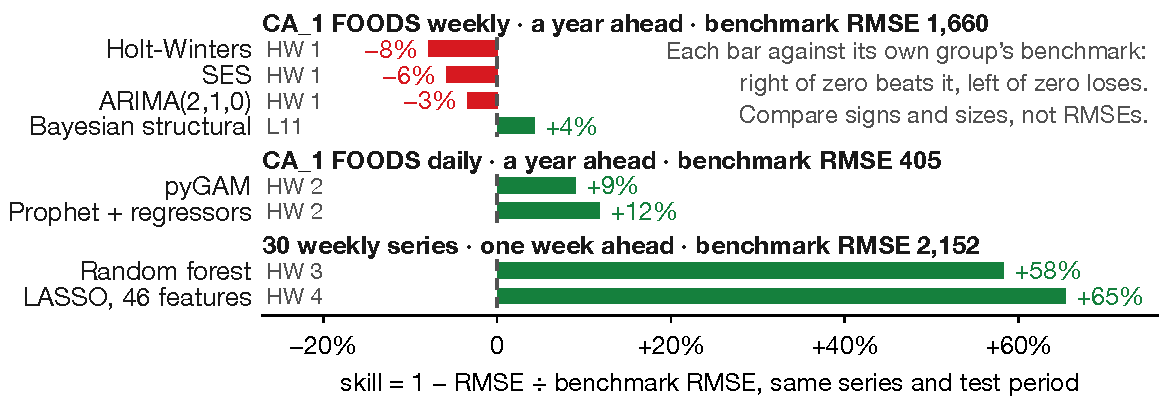
\includegraphics[height=4.1cm]{../Figures/Lecture13_Synthesis/skill_bars.pdf}
  \end{center}
  \vspace{-0.5cm}
  \begin{keybox}
    \textbf{Compute the benchmark first, every time.} It costs one line and says whether
    the rest of the work was worth doing.
  \end{keybox}
\end{frame}

% --- Slide: sophistication -----------------------------------------------------
\begin{frame}{Lesson 2: More Sophisticated Did Not Mean Better}
  Four times this course, the more advanced method failed to win --- and each time for a reason we
  could name.
  \begin{center}
    {\small
    \begin{tabular}{p{3.6cm}p{8.7cm}}
      \toprule
      \textbf{LSTM lost to a plain RNN} & At three windows, \emph{at a fixed 30-epoch budget}; at
      26 weeks they tie by 100 epochs. Gating fixes forgetting, and with 91\% of the variance
      between series there is little to forget. \\[3pt]
      \textbf{Transformer lost to an RNN} & 67{,}329 parameters against roughly \textbf{100
      effectively independent} 52-week blocks --- ours overlap 98\%. \\[3pt]
      \textbf{CNNs lost to LASSO} & Their 26-week window held no annual lag; LASSO was handed one. \\[3pt]
      \textbf{Tuning bought nothing measurable} & Nine fits and a 3-unit change, against a
      \textbf{seed spread of 20--90} at one fixed config. CV improved; test did not. \\
      \bottomrule
    \end{tabular}
    }
  \end{center}

  \vspace{0.05cm}
  \textbf{None of these means the losing method is bad} --- each solves a problem this data does
  not have: long dependency chains, large corpora.
\end{frame}

% --- Slide: sophistication, the picture -----------------------------------------
\begin{frame}{Lesson 2, Continued: A Problem This Data Does Not Have}
  Gates fix forgetting. What does this panel ask a model to remember? Lecture 9's 30 series:
  \begin{center}
    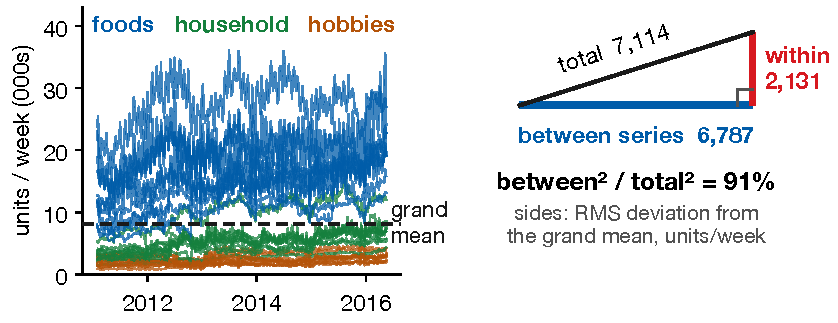
\includegraphics[height=4.0cm]{../Figures/Lecture09_Part1/panel_between_within.pdf}
  \end{center}
  \vspace{-0.3cm}
  \textbf{91\%} of the variance is \emph{which series}, not \emph{which week}: little for a gate
  to keep. Transformers, likewise, earn their parameters on large corpora.

  \begin{keybox}
    \textbf{Match the method to the structure of the problem}, not to the recency of the paper.
  \end{keybox}
\end{frame}

% --- Slide: the recurring idea ---------------------------------------------------
\begin{frame}{Lesson 3: One Idea Appeared Six Times}
  \begin{center}
    {\small
    \begin{tabular}{p{2.0cm}p{4.0cm}p{6.3cm}}
      \toprule
      \textbf{Lecture} & \textbf{Name it went by} & \textbf{What it penalized} \\
      \midrule
      3 & GAM smoothing penalty & Wiggliness of a spline \\
      4 & Cost-complexity pruning & Number of leaves \\
      5 & \texttt{reg\_lambda}, \texttt{gamma} & Leaf weights, leaf count \\
      6 & Ridge, LASSO, Elastic Net & Coefficient size \\
      7 & Weight decay, dropout & Network weights \\
      11 & Hierarchical prior & Distance from the group mean \\
      \bottomrule
    \end{tabular}
    }
  \end{center}

  \vspace{0.05cm}
  Six model families that look nothing alike, one bargain underneath: \textbf{fit against
  complexity, with a single parameter setting the exchange rate.}

  \vspace{0.15cm}
  Five of those six tune that parameter by cross-validation. The sixth --- the hierarchical prior
  --- \textbf{estimates it}, which is the cleanest version of the idea in the course.

  \vspace{0.1cm}
  \textbf{This is what to remember when the tools change.} The libraries in this course will be
  replaced. The trade between fit and complexity will not.
\end{frame}

% =============================================================================
\section{Choosing a Method}
% =============================================================================

\sectionslide{Choosing a Method}{%
  A decision guide built from what we measured.}

% --- Slide: decision guide --------------------------------------------------------
\begin{frame}{Which Method, When}
  \begin{center}
    {\small
    \begin{tabular}{p{4.6cm}p{7.7cm}}
      \toprule
      \textbf{If your situation is\ldots} & \textbf{start here} \\
      \midrule
      One series, clear seasonality, short history & ETS or ARIMA --- and check the benchmark \\[1pt]
      Several seasonal cycles at once & GAM or Prophet \\[1pt]
      Many engineered features, tabular & \textbf{Regularized regression first}, then XGBoost \\[1pt]
      Many parallel series, shared drivers & Gradient boosting with series identifiers \\[1pt]
      Genuinely long dependencies, lots of data & Recurrent or attention architectures \\[1pt]
      Few observations per group & Hierarchical Bayesian --- partial pooling \\[1pt]
      The decision needs a probability & Bayesian, for the predictive distribution \\
      \bottomrule
    \end{tabular}
    }
  \end{center}

  \vspace{0.05cm}
  ``Regularized regression first'' is not a concession --- it won our largest comparison and its
  coefficients can be read aloud. And the last row is the only one where the \emph{question}
  changes rather than the accuracy.
\end{frame}

% =============================================================================
\section{Doing It Honestly}
% =============================================================================

\sectionslide{Doing It Honestly}{%
  The errors in this field do not announce themselves.}

% --- Slide: silent errors ----------------------------------------------------------
\begin{frame}{Errors That Fail Silently I: the Pipeline}
  Confident, plausible, wrong and silent --- and every one a \textbf{bug in the code}.
  \begin{center}
    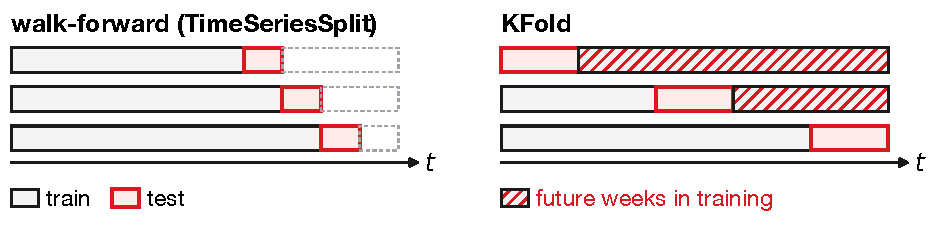
\includegraphics[height=2.8cm]{../Figures/Lecture13_Synthesis/cv_splits.pdf}
  \end{center}
  \vspace{-0.15cm}
  \begin{center}
    {\small
    \begin{tabular}{p{3.9cm}p{9.6cm}}
      \toprule
      \texttt{KFold} on a time series & Future weeks train the model; CV looks great, the
      forecast fails. \\
      Scaling outside the fold & Validation statistics leak into training. \\
      Rolling features unshifted & The current week leaks the target into its own predictor. \\
      Reading MDI importance & Noise ranked \textbf{17th of 29} in Homework 3 on distinct
      values alone. \\
      \bottomrule
    \end{tabular}
    }
  \end{center}

  \vspace{-0.1cm}
  \textbf{Not a crash but a number that looks fine}, so the discipline is procedural: split by
  time, scale inside the fold, shift the window, plant a control.
\end{frame}

% --- Slide: silent failures II ------------------------------------------------------
\begin{frame}{Errors That Fail Silently II: the Code Was Fine}
  Harder, and more common in professional work. Here \textbf{nothing is wrong with the program}:
  the model fits, the diagnostics pass, and the answer is still wrong.
  \begin{center}
    {\small
    \begin{tabular}{p{3.7cm}p{8.6cm}}
      \toprule
      Pooling groups that are not \textbf{exchangeable} & Lecture 11 Part 2 pooled ten FOODS
      series with twenty that ignore SNAP. Textbook shrinkage, clean diagnostics, and it reported
      $+0.011$ where held-out weeks said $+0.089$. \\[3pt]
      Standardizing a coefficient you then \textbf{interpret} & Lecture 12: divide log price by
      its standard deviation and \texttt{b\_price} stops being an elasticity. Identical fit,
      identical diagnostics, and the 5\% price scenario moves by \textbf{22$\times$}. \\[3pt]
      Omitting a confounder & The naive elasticity was six times too large \emph{with an interval
      half the width}. Precision is not accuracy. \\[3pt]
      Ignoring $\hat{R}$ and divergences & Our first two Bayesian fits returned
      reasonable-looking forecasts while failing convergence outright. \\
      \bottomrule
    \end{tabular}
    }
  \end{center}

  \vspace{-0.05cm}
  \textbf{Only the last row has a diagnostic.} The first three were caught by held-out data, by a
  DAG drawn before the model, and by asking what one unit of a variable means --- none of which
  any library will run for you.
\end{frame}

% --- Slide: the day every model fails ----------------------------------------------
\begin{frame}{The Day Every Model in This Course Fails}
  Every 25 December the stores close and sales are \textbf{exactly zero}. CA\_1 FOODS, 2012--15:
  \begin{center}
    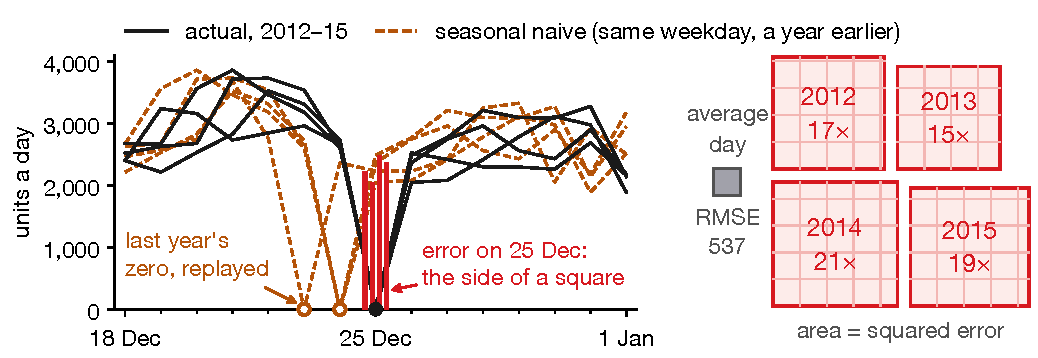
\includegraphics[height=3.7cm]{../Figures/Lecture13_Synthesis/christmas_squares.pdf}
  \end{center}
  \vspace{-0.3cm}
  Four days, \textbf{0.25\%} of the evaluation window, carry \textbf{4.6\%} of its squared error.
  Yet \texttt{is\_event} fires on \textbf{158} days, only \textbf{5} of them closures.

  \begin{keybox}
    Knowable years ahead, and every method failed: the \emph{encoding}, not the model, lumped a
    locked door in with the Super Bowl.
  \end{keybox}
\end{frame}

% --- Slide: what to report ---------------------------------------------------------
\begin{frame}{What a Defensible Forecast Report Contains}
  \begin{center}
    {\small
    \begin{tabular}{p{3.4cm}p{8.9cm}}
      \toprule
      \textbf{A benchmark} & Computed, not cited. Every model measured against it. \\[2pt]
      \textbf{A time-aware split} & Walk-forward or a held-out final block, never random. \\[2pt]
      \textbf{More than one evaluation} & A single test split can flatter. Homework 4 ranked
      models the same way twice, which is why that ranking is believable. \\[2pt]
      \textbf{The result that went against you} & Including tuning that did not help, and the
      model you expected to win. \\[2pt]
      \textbf{An interpretation} & In the units of the business, not of the loss function. \\
      \bottomrule
    \end{tabular}
    }
  \end{center}

  \vspace{0.05cm}
  \textbf{The fourth row is the one that distinguishes professional work.} A report where every
  result confirms the author's expectation is not a report anyone should act on.

  \vspace{0.1cm}
  You have practised this all semester: the assignments were built so the obvious answer is
  frequently the wrong one, and the credit was for noticing.
\end{frame}

% --- Slide: the final project -------------------------------------------------------
\begin{frame}{Where You Do This Yourself}
  The final project asks for exactly the report on the previous slide, on data of your choosing.

  \begin{center}
    {\small
    \begin{tabular}{p{3.6cm}p{8.7cm}}
      \toprule
      \textbf{Three methods, from at least two parts of the course} & Classical, trees, deep
      learning, Bayesian. Three variations on one family does not count --- the comparison must be
      between approaches differing \emph{in kind}. \\[3pt]
      \textbf{Plus a benchmark} & Which does not count toward the three, and is not optional.
      Lesson 1 is why. \\[3pt]
      \textbf{Walk-forward validation} & For every comparison. Not a random split, not once. \\[3pt]
      \textbf{A recommendation a non-specialist can act on} & In the units of the business, with
      the uncertainty attached. \\[3pt]
      \textbf{A methods reflection} & Which model won, and what about \emph{your} data made it
      win. This is where the course is actually assessed. \\
      \bottomrule
    \end{tabular}
    }
  \end{center}

  \vspace{-0.05cm}
  \textbf{The last row is not a formality.} Every scoreboard in this course came with a reason,
  and a project that reports a ranking without one has done the computation but not the work.
\end{frame}

% =============================================================================
\section{Where to Go Next}
% =============================================================================

\sectionslide{Where to Go Next}{%
  What we left out, and what to read.}

% --- Slide: not covered ------------------------------------------------------------
\begin{frame}{What This Course Did Not Cover}
  \begin{columns}[T]
    \begin{column}{0.64\textwidth}
      {\small
      \begin{tabular}{@{}>{\raggedright\arraybackslash}p{2.6cm}>{\raggedright\arraybackslash}p{6.2cm}@{}}
        \toprule
        \textbf{Hierarchical reconciliation} & Store forecasts that add up to regional totals.
        FPP Ch.~11. \\[4pt]
        \textbf{Intermittent demand} & Mostly-zero series: Croston's method and its
        relatives. \\[4pt]
        \textbf{Structural breaks} & The future stops resembling the past, and every method
        fails together. \\[4pt]
        \textbf{Causal inference} & DAGs told us confounders exist; credible causal estimates
        are a separate course. \\[4pt]
        \textbf{Foundation models} & Pretrained forecasters, zero-shot. FPP-Py Ch.~15 is a
        start. \\
        \bottomrule
      \end{tabular}
      }
    \end{column}
    \begin{column}{0.33\textwidth}
      \centering
      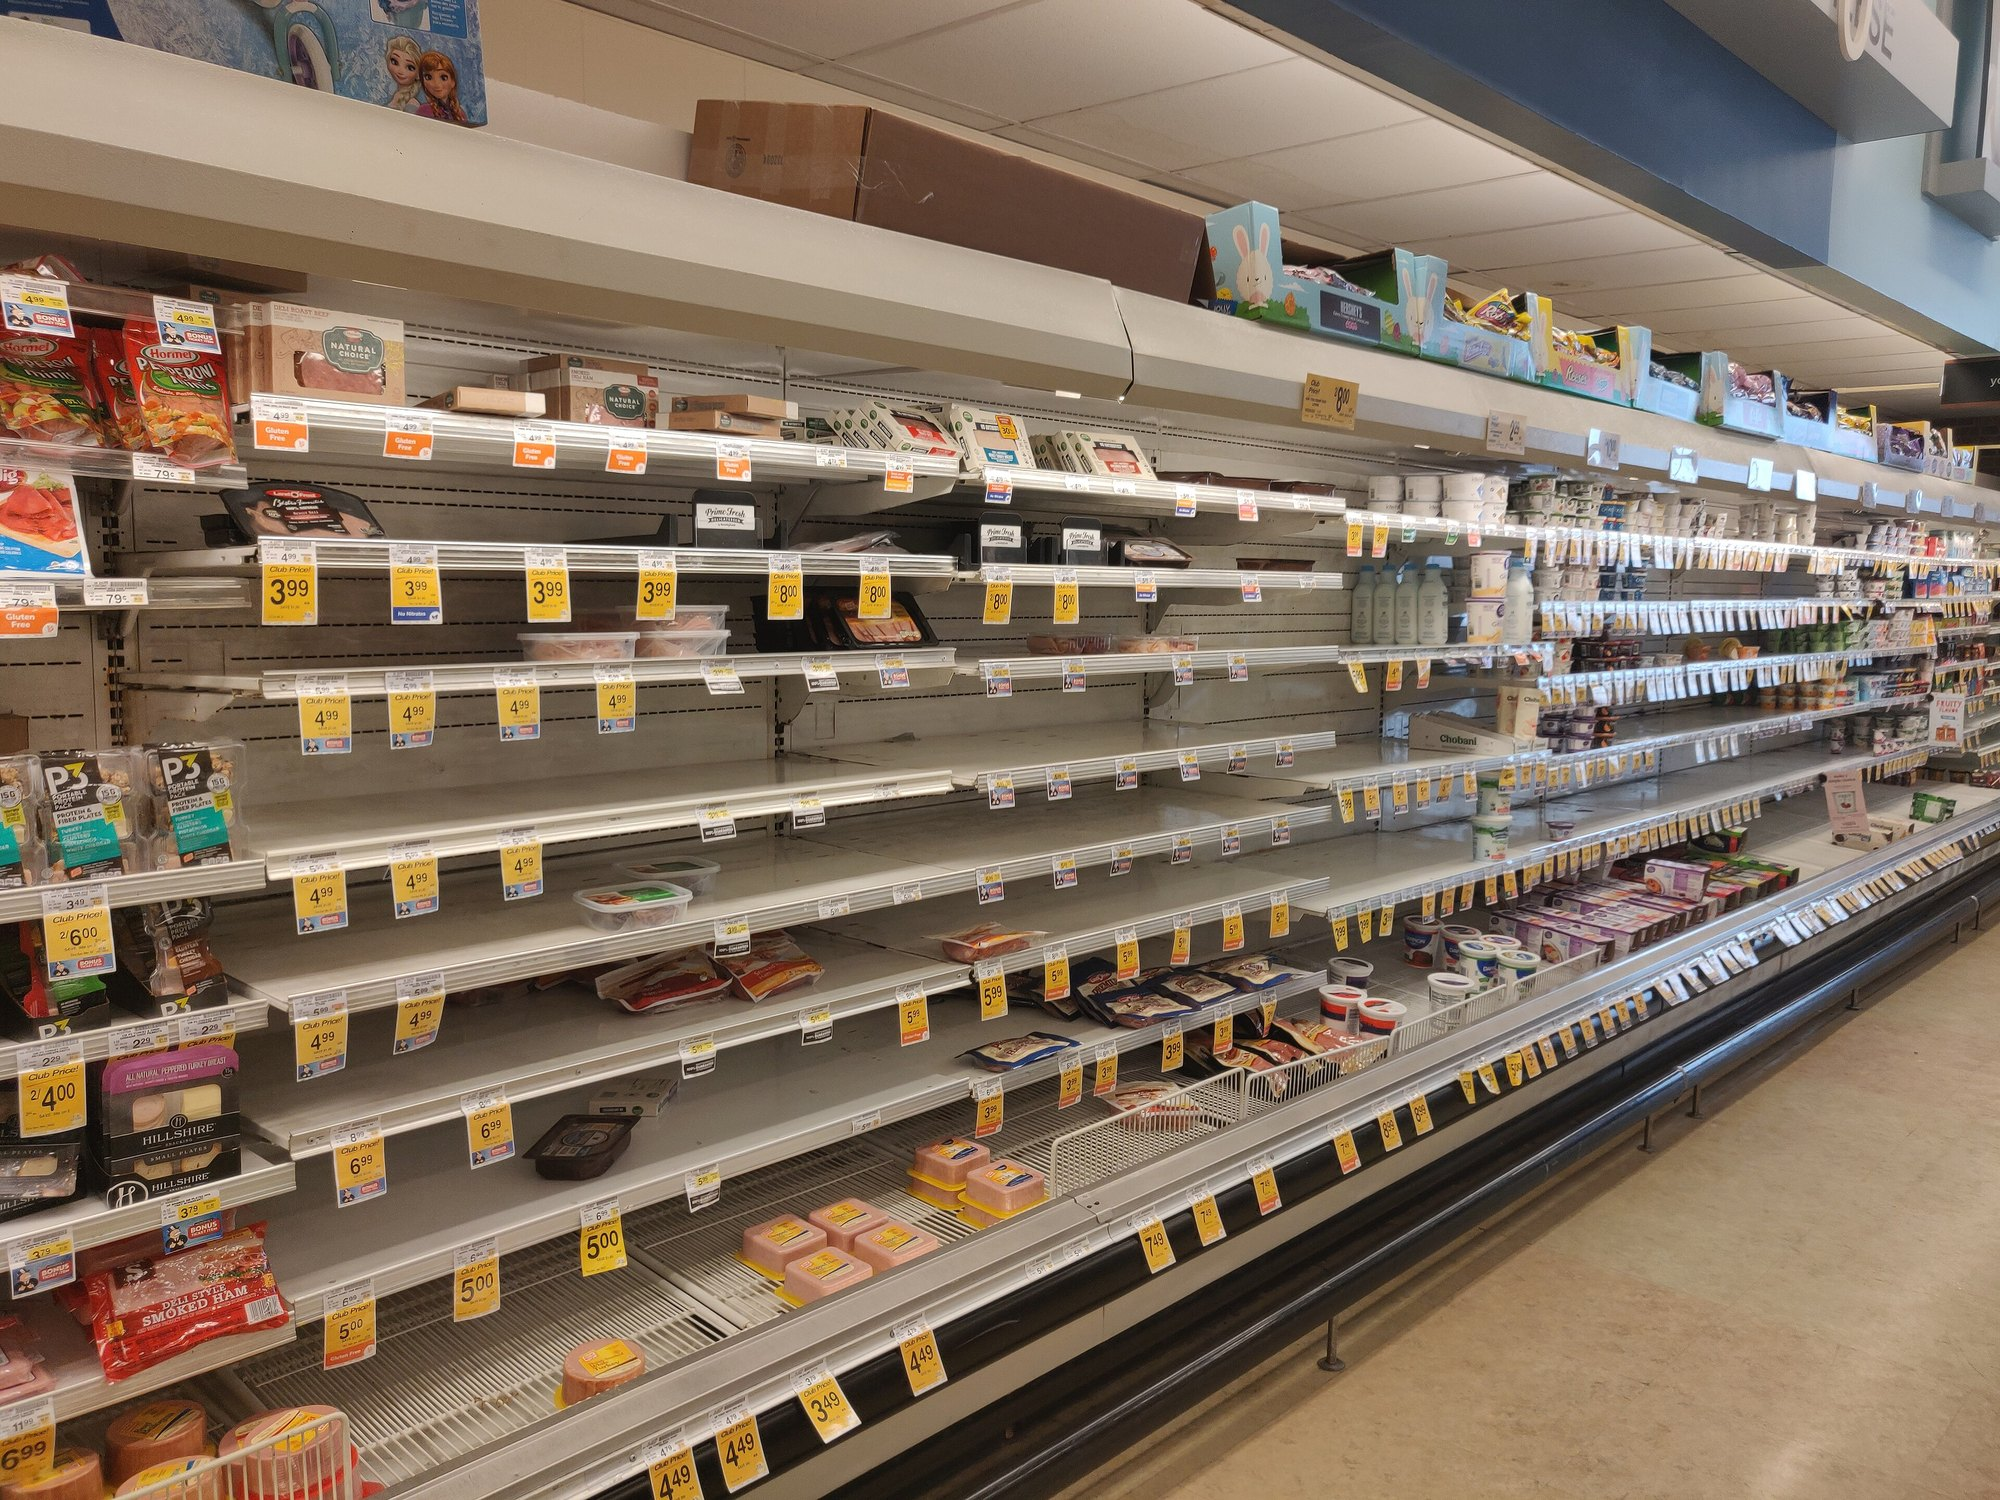
\includegraphics[width=\linewidth]{../Figures/Lecture08/source/aisle-march-2020.jpg}\\[1pt]
      {\scriptsize\color{unogray} Washington, DC, 18~March 2020. Photo: Kurt Kaiser (CC0).\par}
    \end{column}
  \end{columns}

  \vspace{0.25cm}
  \textbf{The third row is the one most likely to matter in your career.} Every model here
  assumes the future resembles the past. When it stops, the model does not tell you --- and the
  benchmark fails at the same moment.
\end{frame}

% --- Slide: closing ------------------------------------------------------------------
\begin{frame}{Closing}
  \begin{keybox}
    {\small
    \begin{enumerate}\itemsep3pt
      \item \textbf{Compute the benchmark first.} It says whether the rest was worth doing.
      \item \textbf{Match the method to the problem}: our most advanced finished fifth.
      \item \textbf{One idea recurs:} fit against complexity, one parameter setting the rate.
      \item \textbf{Split by time, always.} Leakage does not crash; it flatters.
      \item \textbf{Diagnostics check the model, not the question.} Held-out data caught our worst two.
      \item \textbf{Report what went against you.}
      \item \textbf{Know what the forecast is for.} Decisions need a distribution.
    \end{enumerate}
    }
  \end{keybox}

  \vspace{0.05cm}
  \muted{\itshape The libraries will change. The habits are the transferable part.}
\end{frame}

\begin{frame}[allowframebreaks]{References}
  \printbibliography[heading=none]
\end{frame}

\end{document}
